% для компиляции в lualatex!!
%\documentclass[12pt, a4paper]{article}
\documentclass[12pt, a4paper]{disser}
\usepackage[english,russian]{babel}
\usepackage[warn]{mathtext}
%\usepackage[T2A]{fontenc}
%\usepackage[utf8]{inputenc}

\usepackage{xecyr} % Продукт Вашего покорного слуги ;)

%\setmainfont{DejaVu Serif}
\setmainfont{Liberation Serif}

\usepackage{color}
\usepackage{amssymb,amsmath}
\usepackage{graphicx}
\usepackage{multicol}

\textheight=24cm           % высота текста
\textwidth=16cm            % ширина текста
\oddsidemargin=0pt         % отступ от левого края
\topmargin=-1.5cm          % отступ от верхнего края
\parindent=24pt            % абзацный отступ
\parskip=0pt               % интервал между абзацами
\tolerance=2000            % терпимость к "жидким" строкам
\flushbottom               % выравнивание высоты страниц
%\def\baselinestretch{1.5} % печать с большим интервалом

%\title{}
%\author{\copyright~~С.А.~Назарова \thanks{e-mail:~sophia.nazarova@gmail.com}}
%\date{}

\begin{document}
	\begin{figure}[h]

	\begin{minipage}[b]{.46\linewidth}
%Фигурка в первом ряду слева размер отведенный под весь этот объект \textendash 0.46 от ширины строки
%Параметр [b] означает, что выравнивание этих министраниц будет по нижнему краю
	\begin{center}
%	{\small N~{\it Macoma balthica}}
		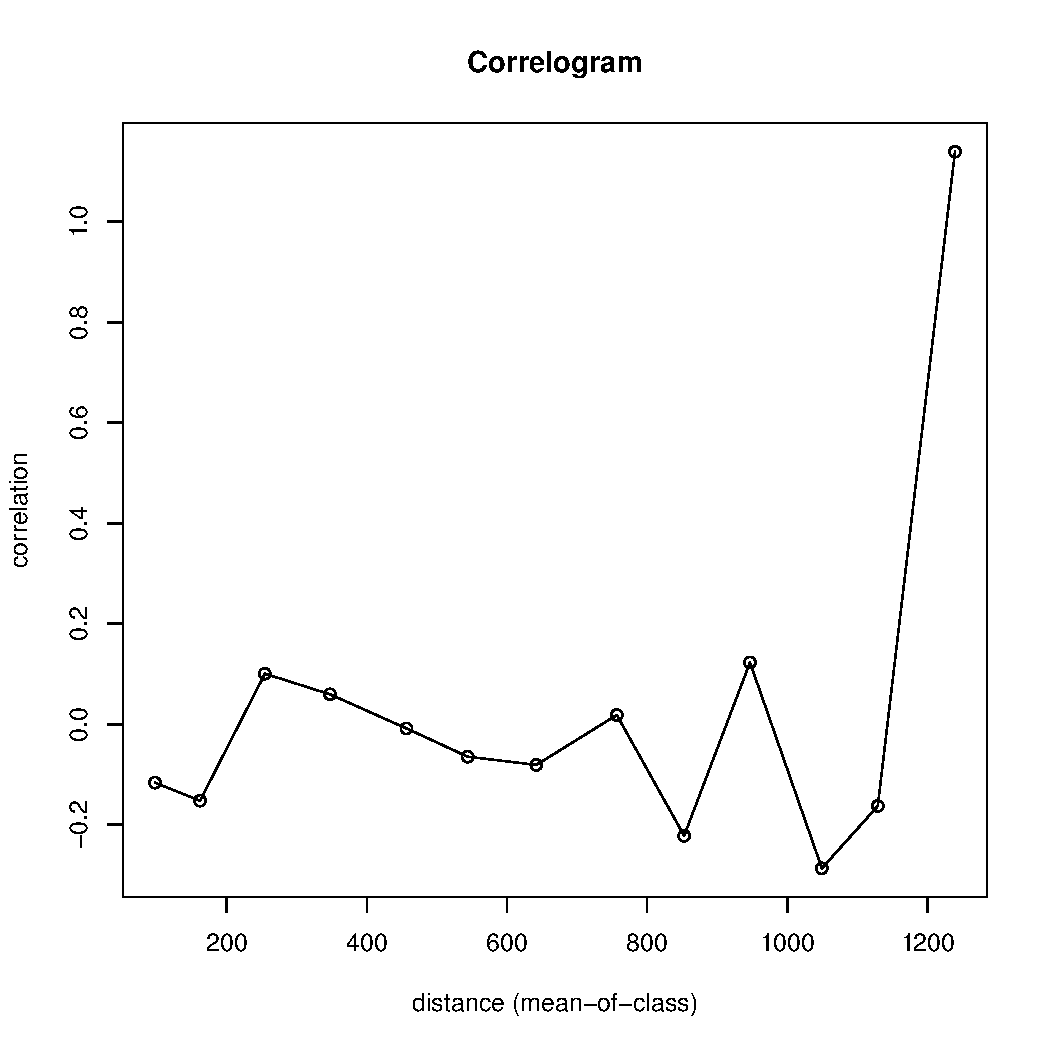
\includegraphics[width=65mm]{./Pala_macoma_age_N1_.pdf}
	\end{center}
	\end{minipage}
%
	\hfil %Это пружинка отодвигающая рисунки друг от друга
%
	\begin{minipage}[b]{.46\linewidth}
%Следующий рисунок - первый ряд справа %DUNGEON S_4 \ AB
	\begin{center}
%	{\small B~{\it Macoma balthica}}
		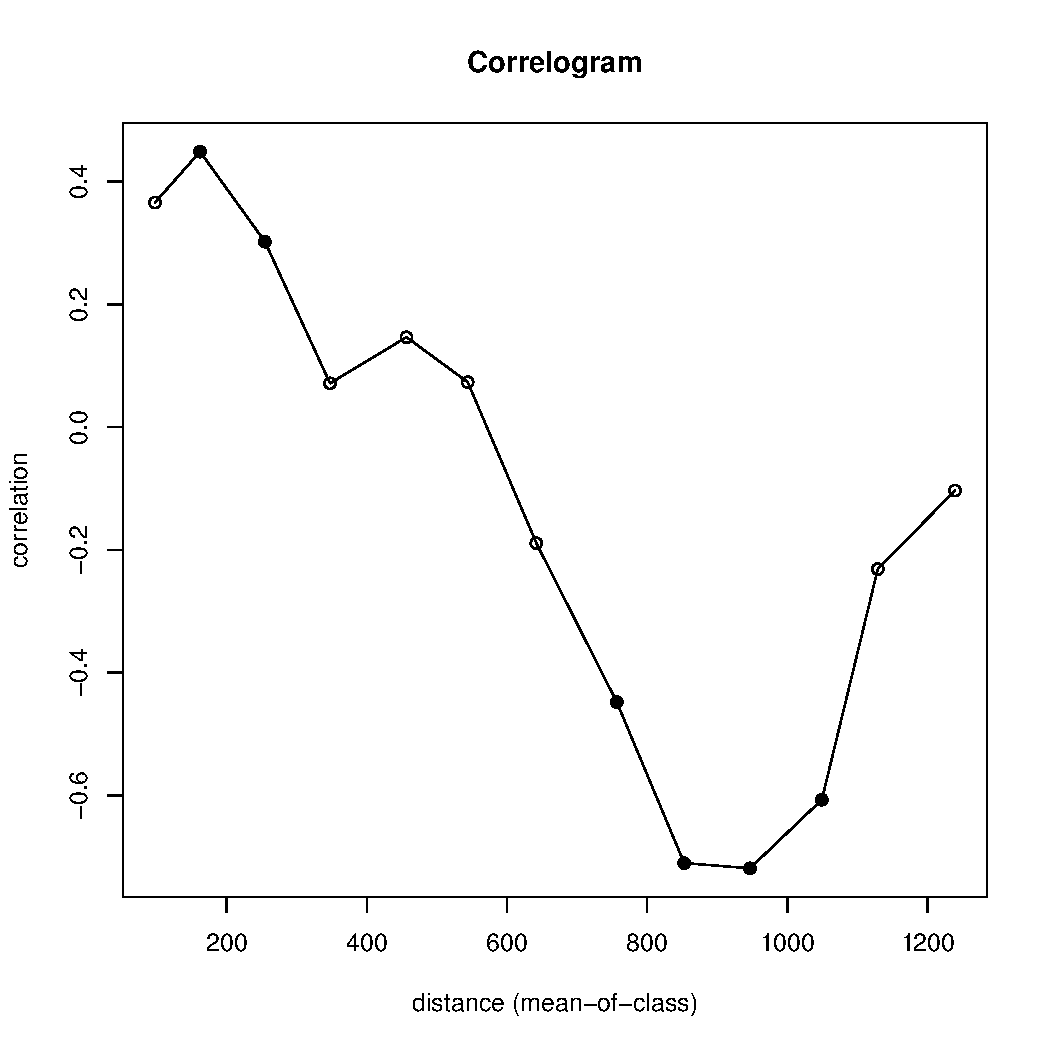
\includegraphics[width=65mm]{./Pala_macoma_age_N2_.pdf}
	\end{center}
	\end{minipage}

	
	\begin{minipage}[b]{.46\linewidth}
	%Фигурка в первом ряду слева размер отведенный под весь этот объект \textendash 0.46 от ширины строки
	%Параметр [b] означает, что выравнивание этих министраниц будет по нижнему краю
	\begin{center}
%	{\small N~{\it Cerastoderma edule}}
		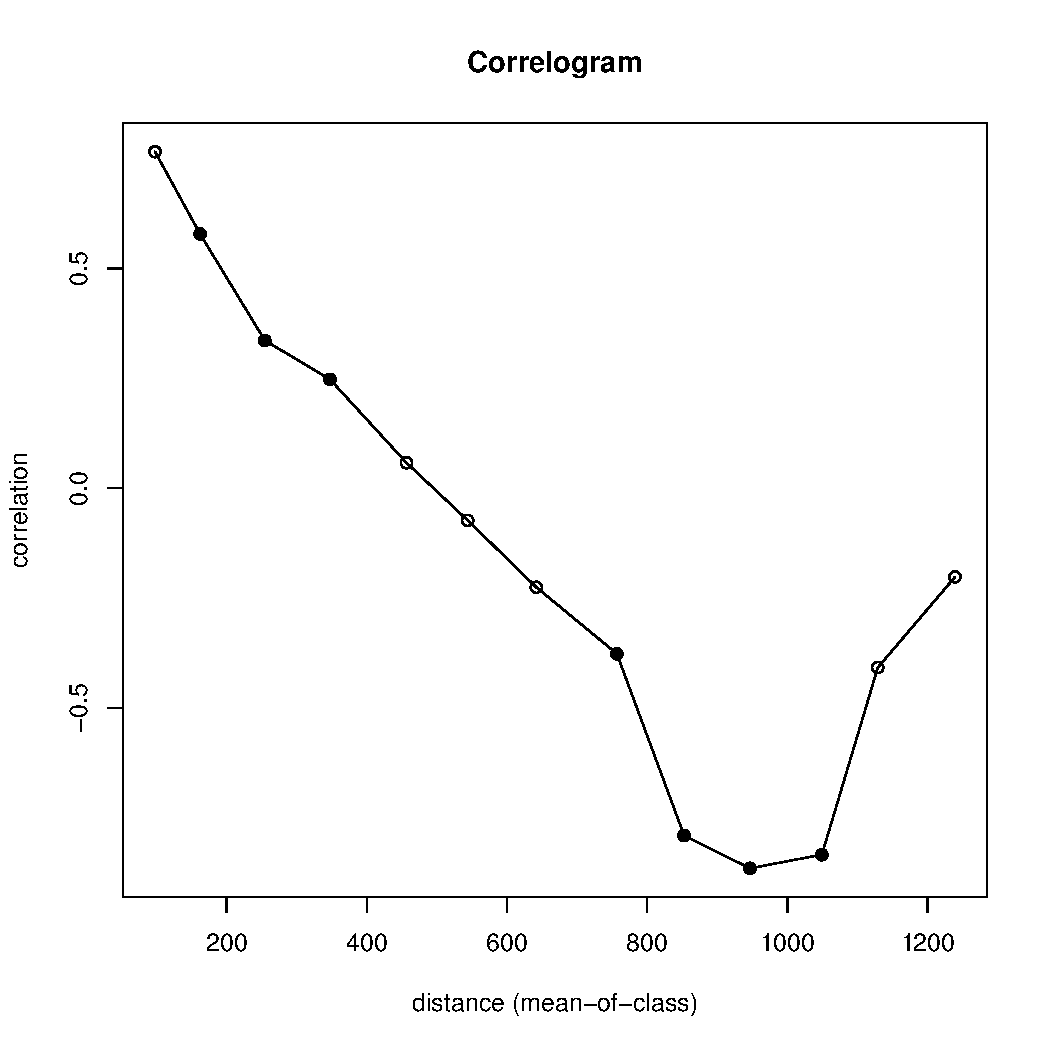
\includegraphics[width=65mm]{./Pala_macoma_age_N3_.pdf}
	\end{center}
	\end{minipage}
	%
	\hfil %Это пружинка отодвигающая рисунки друг от друга
	%
	\begin{minipage}[b]{.46\linewidth}
%Следующий рисунок - первый ряд справа %DUNGEON S_4 \ AB
	\begin{center}
%	{\small B~{\it Cerastoderma edule}}
		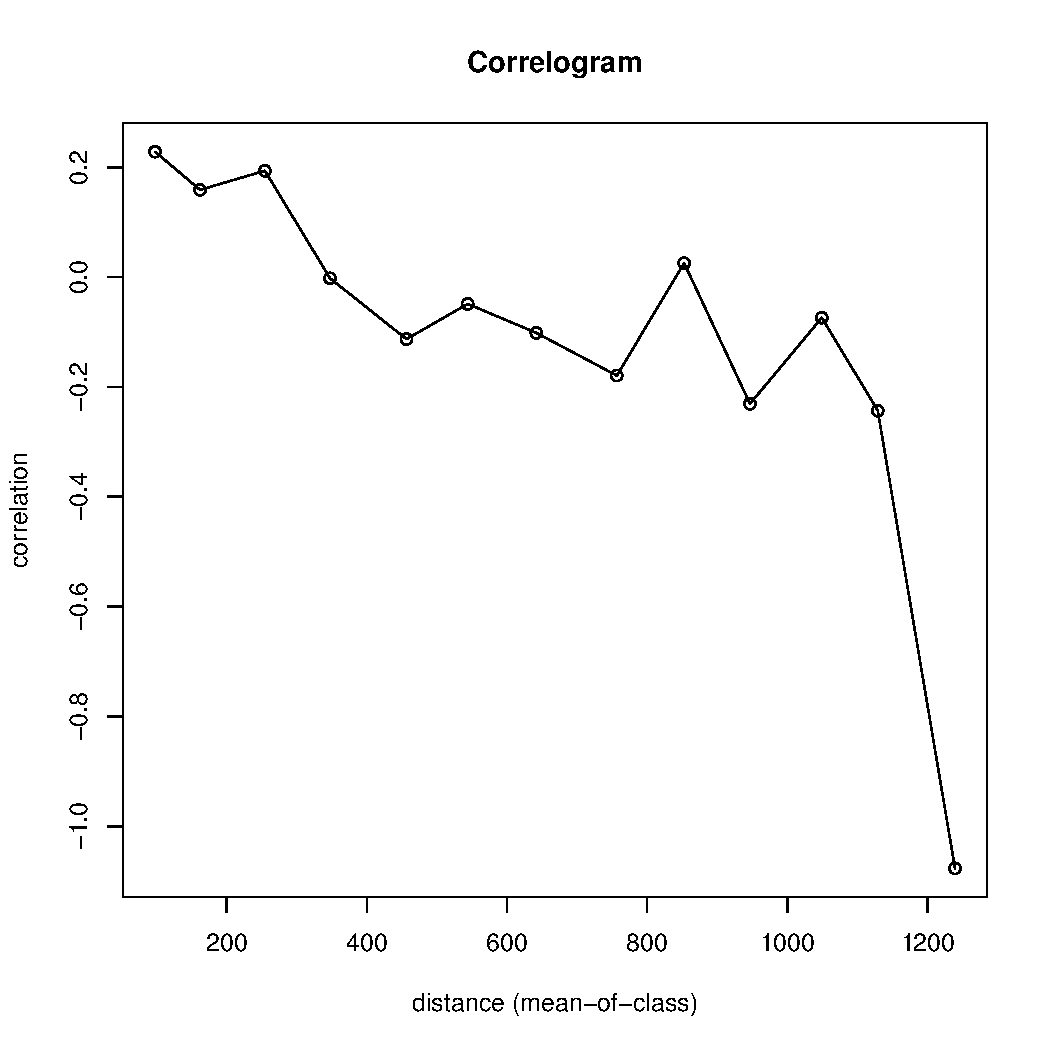
\includegraphics[width=65mm]{./Pala_macoma_age_N4_.pdf}
	\end{center}
	\end{minipage}

%\smallskip



%\smallskip

	\begin{minipage}[b]{.46\linewidth}
%Фигурка в первом ряду слева размер отведенный под весь этот объект \textendash 0.46 от ширины строки
%Параметр [b] означает, что выравнивание этих министраниц будет по нижнему краю
	\begin{center}
%	{\small N~{\it Priapulus caudatus}}
		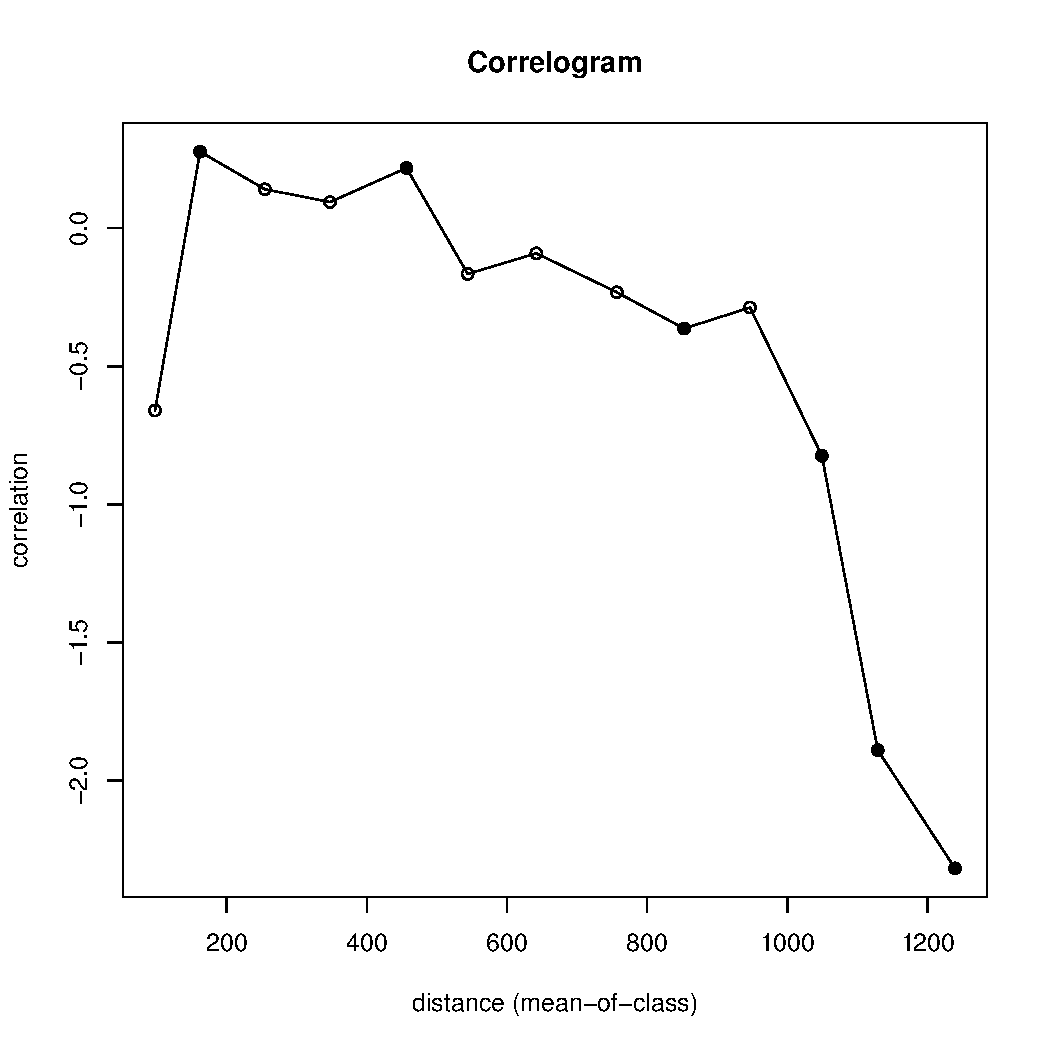
\includegraphics[width=65mm]{./Pala_macoma_age_N5_.pdf}
	\end{center}
	\end{minipage}
%
	\hfil %Это пружинка отодвигающая рисунки друг от друга
%
	\begin{minipage}[b]{.46\linewidth}
%Следующий рисунок - первый ряд справа %DUNGEON S_4 \ AB
	\begin{center}
%	{\small B~{\it Priapulus caudatus}}
		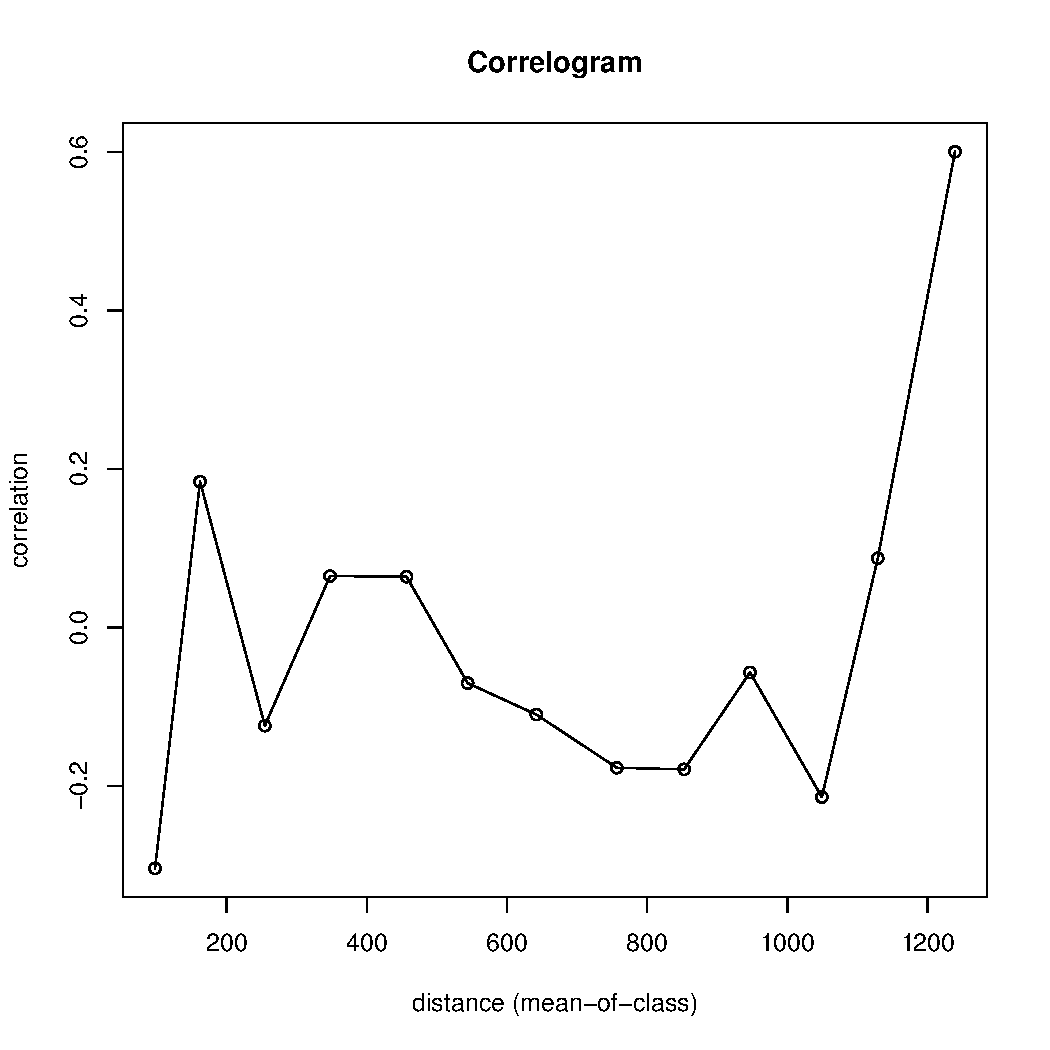
\includegraphics[width=65mm]{./Pala_macoma_age_N6_.pdf}
	\end{center}
	\end{minipage}

%\smallskip


%	\caption{Микрораспределение макробентоса на литорали Пала-губы}
%	\label{ris:moransI_Pala}
	\end{figure}



	\begin{figure}[h]

	\begin{minipage}[b]{.46\linewidth}
%Фигурка в первом ряду слева размер отведенный под весь этот объект \textendash 0.46 от ширины строки
%Параметр [b] означает, что выравнивание этих министраниц будет по нижнему краю
	\begin{center}
%	{\small N~{\it Crangon crangon}}
		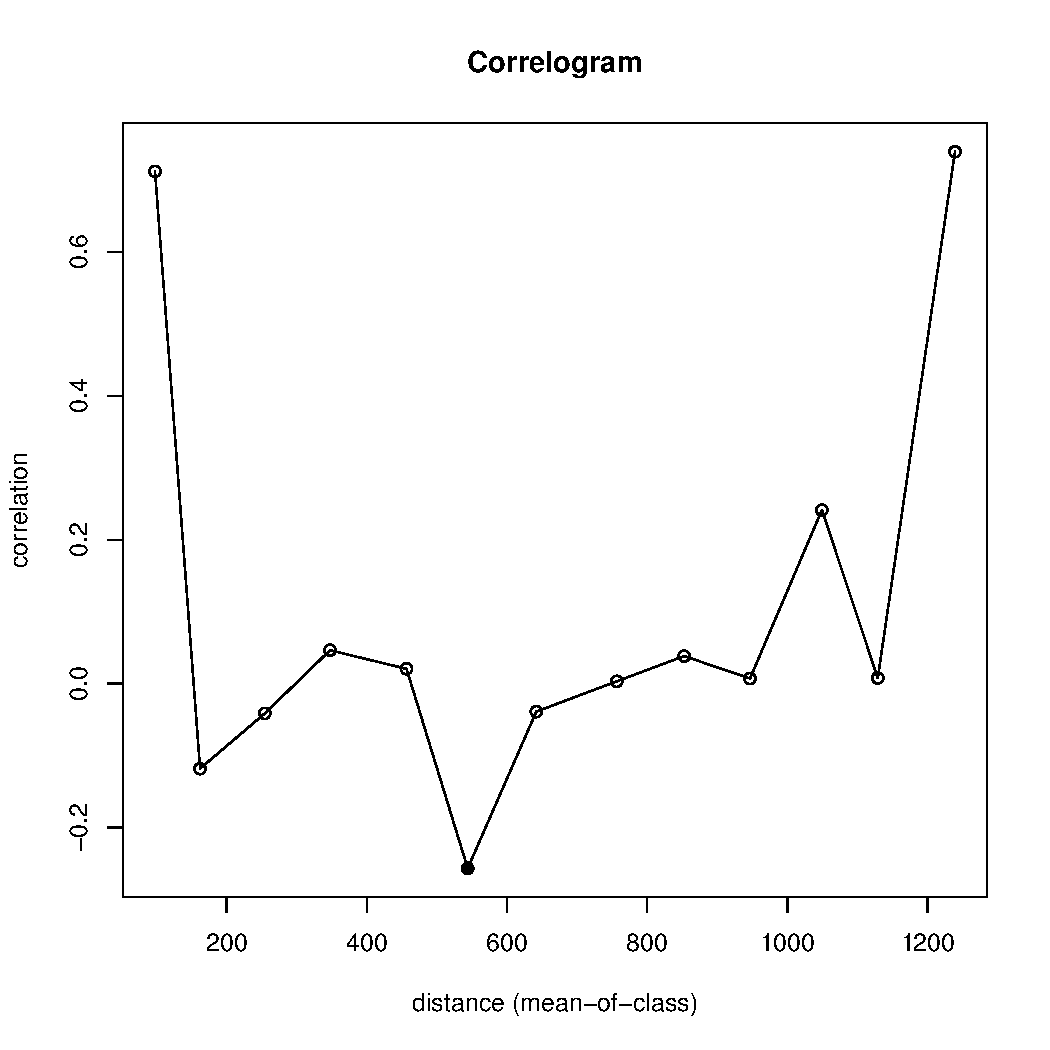
\includegraphics[width=65mm]{./Pala_macoma_age_N7_.pdf}
	\end{center}
	\end{minipage}
%
	\hfil %Это пружинка отодвигающая рисунки друг от друга
%
	\begin{minipage}[b]{.46\linewidth}
%Следующий рисунок - первый ряд справа %DUNGEON S_4 \ AB
	\begin{center}
		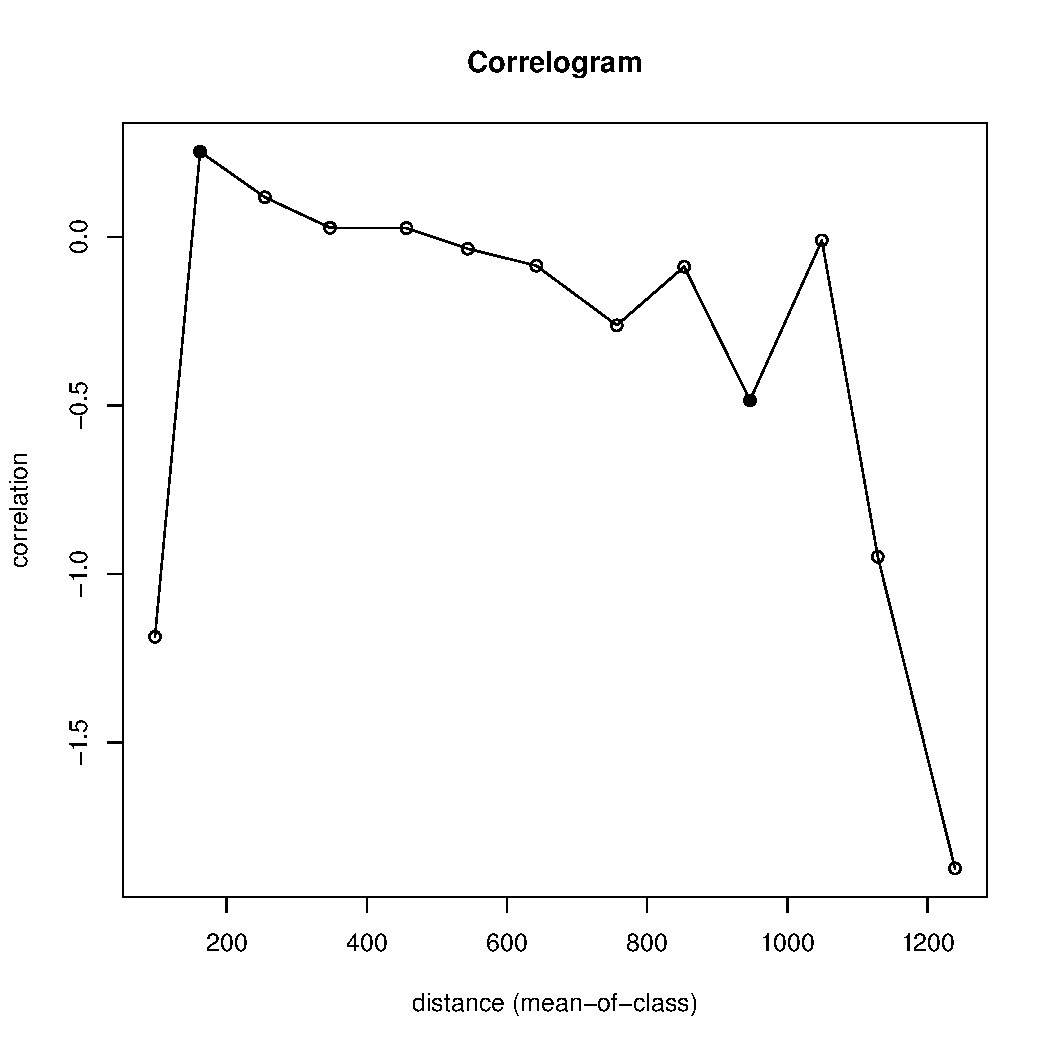
\includegraphics[width=65mm]{./Pala_macoma_age_N8_.pdf}
%	{\small B~{\it Crangon crangon}}
	\end{center}
	\end{minipage}

	
	\begin{minipage}[b]{.46\linewidth}
	%Фигурка в первом ряду слева размер отведенный под весь этот объект \textendash 0.46 от ширины строки
	%Параметр [b] означает, что выравнивание этих министраниц будет по нижнему краю
	\begin{center}
	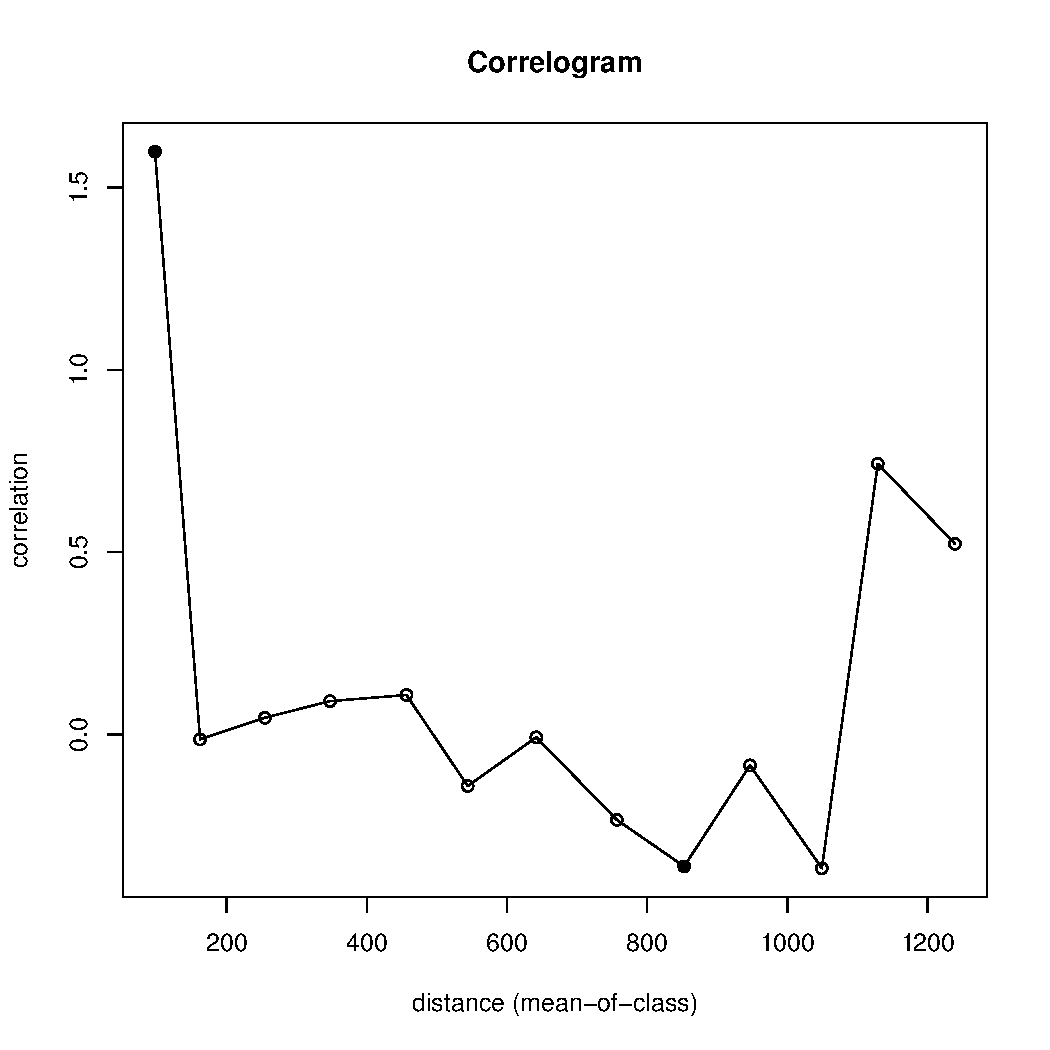
\includegraphics[width=65mm]{./Pala_macoma_age_N9_.pdf}

	\end{center}
	\end{minipage}
	%
	\hfil %Это пружинка отодвигающая рисунки друг от друга
	%
	\begin{minipage}[b]{.46\linewidth}
%Следующий рисунок - первый ряд справа %DUNGEON S_4 \ AB
	\begin{center}
		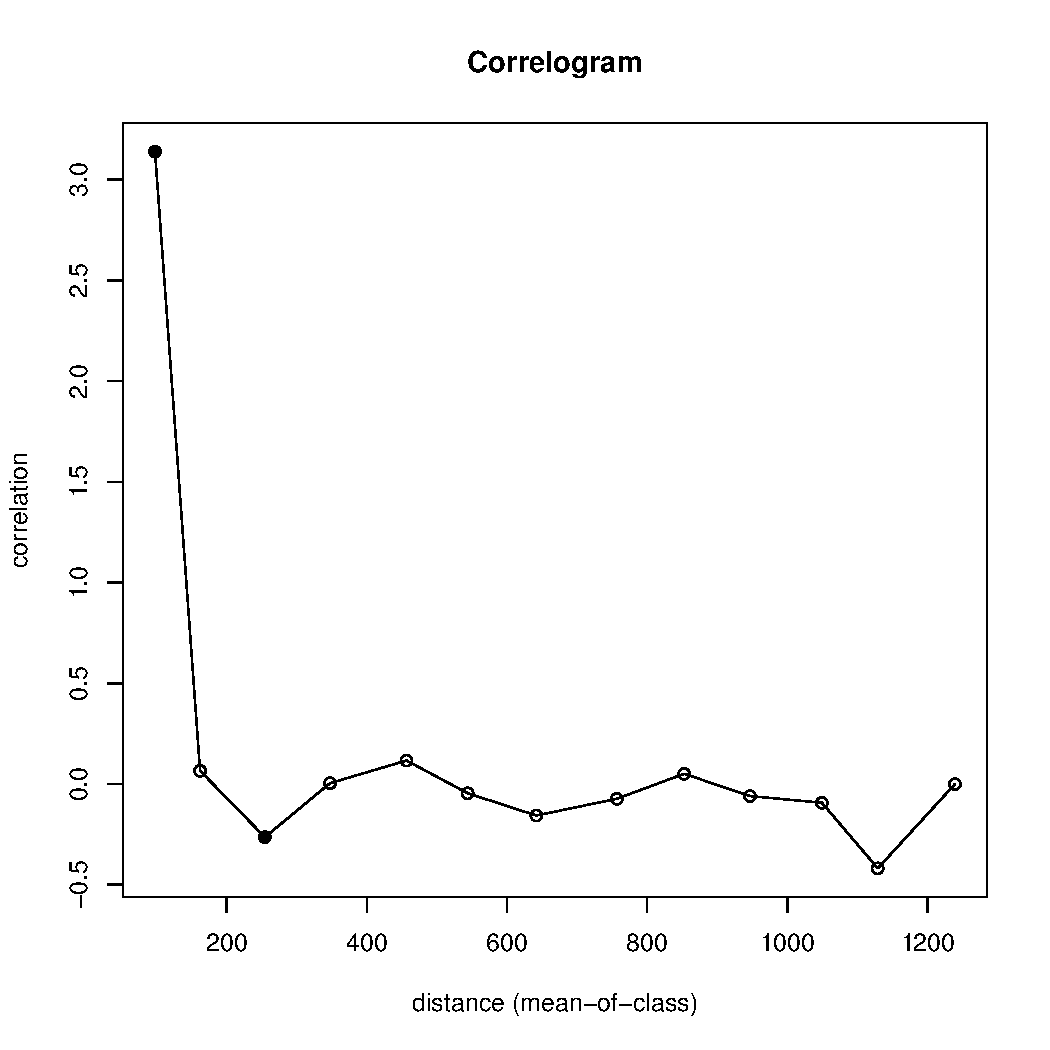
\includegraphics[width=65mm]{./Pala_macoma_age_N10_.pdf}
	\end{center}
	\end{minipage}

%\smallskip



%\smallskip

	\begin{minipage}[b]{.46\linewidth}
%Фигурка в первом ряду слева размер отведенный под весь этот объект \textendash 0.46 от ширины строки
%Параметр [b] означает, что выравнивание этих министраниц будет по нижнему краю
	\begin{center}
		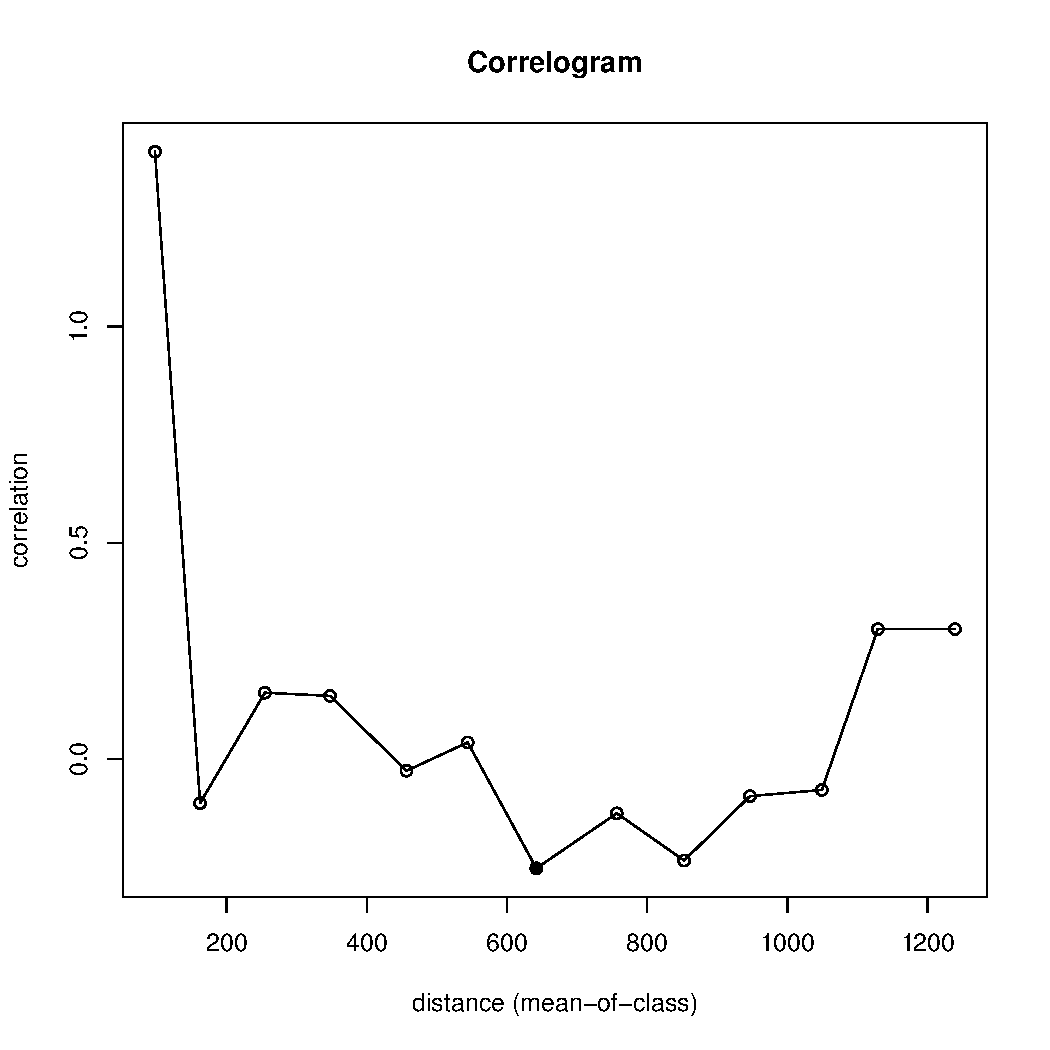
\includegraphics[width=65mm]{./Pala_macoma_age_N11_.pdf}
	\end{center}
	\end{minipage}
%
	\hfil %Это пружинка отодвигающая рисунки друг от друга
%
	\begin{minipage}[b]{.46\linewidth}
%Следующий рисунок - первый ряд справа %DUNGEON S_4 \ AB
	\begin{center}
		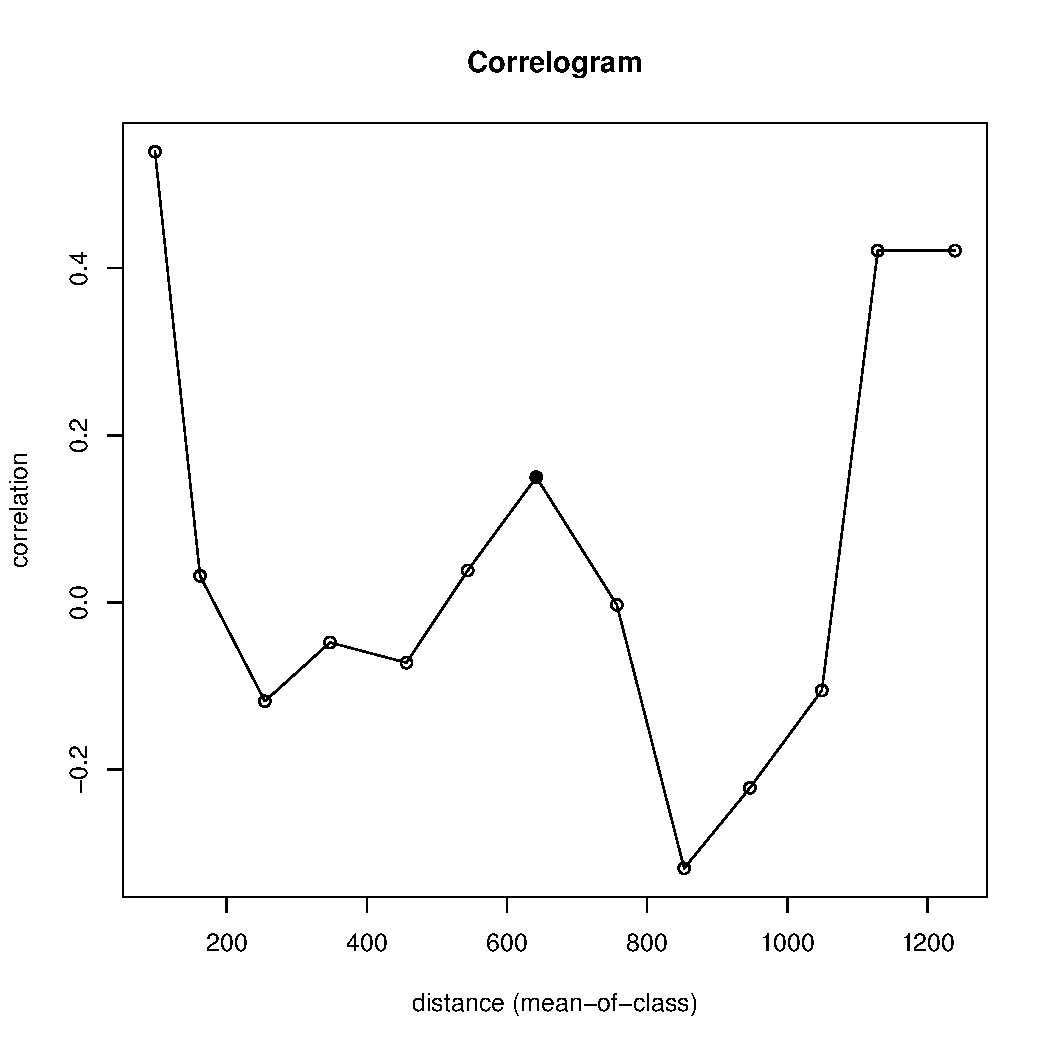
\includegraphics[width=65mm]{./Pala_macoma_age_N12_.pdf}
	\end{center}
	\end{minipage}

%\smallskip



%	\caption{Микрораспределение макробентоса на литорали Пала-губы (Продолжение)}
%	\label{ris:moransI_Pala}
%	\begin{center}
%	Рис. \ref{ris:moransI_Pala} (продолжение). Микрораспределение макробентоса на литорали Пала-губы.
%	\end{center}

	\end{figure}



	\begin{figure}[h]

	\begin{minipage}[b]{.46\linewidth}
%Фигурка в первом ряду слева размер отведенный под весь этот объект \textendash 0.46 от ширины строки
%Параметр [b] означает, что выравнивание этих министраниц будет по нижнему краю
	\begin{center}
%	{\small N~{\it Macoma balthica}}
		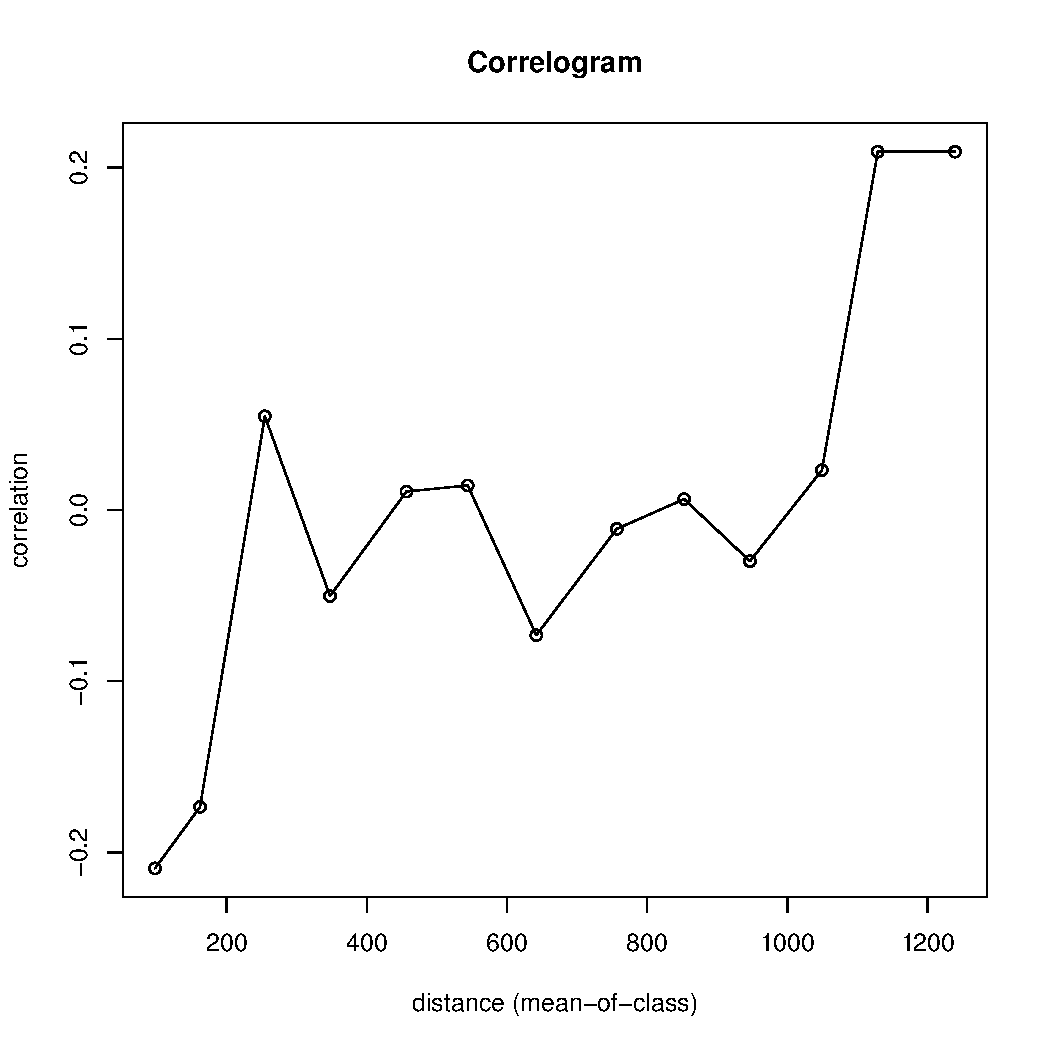
\includegraphics[width=65mm]{./Pala_macoma_age_N13_.pdf}
	\end{center}
	\end{minipage}
%
	\hfil %Это пружинка отодвигающая рисунки друг от друга
%
	\begin{minipage}[b]{.46\linewidth}
%Следующий рисунок - первый ряд справа %DUNGEON S_4 \ AB
	\begin{center}
%	{\small B~{\it Macoma balthica}}
		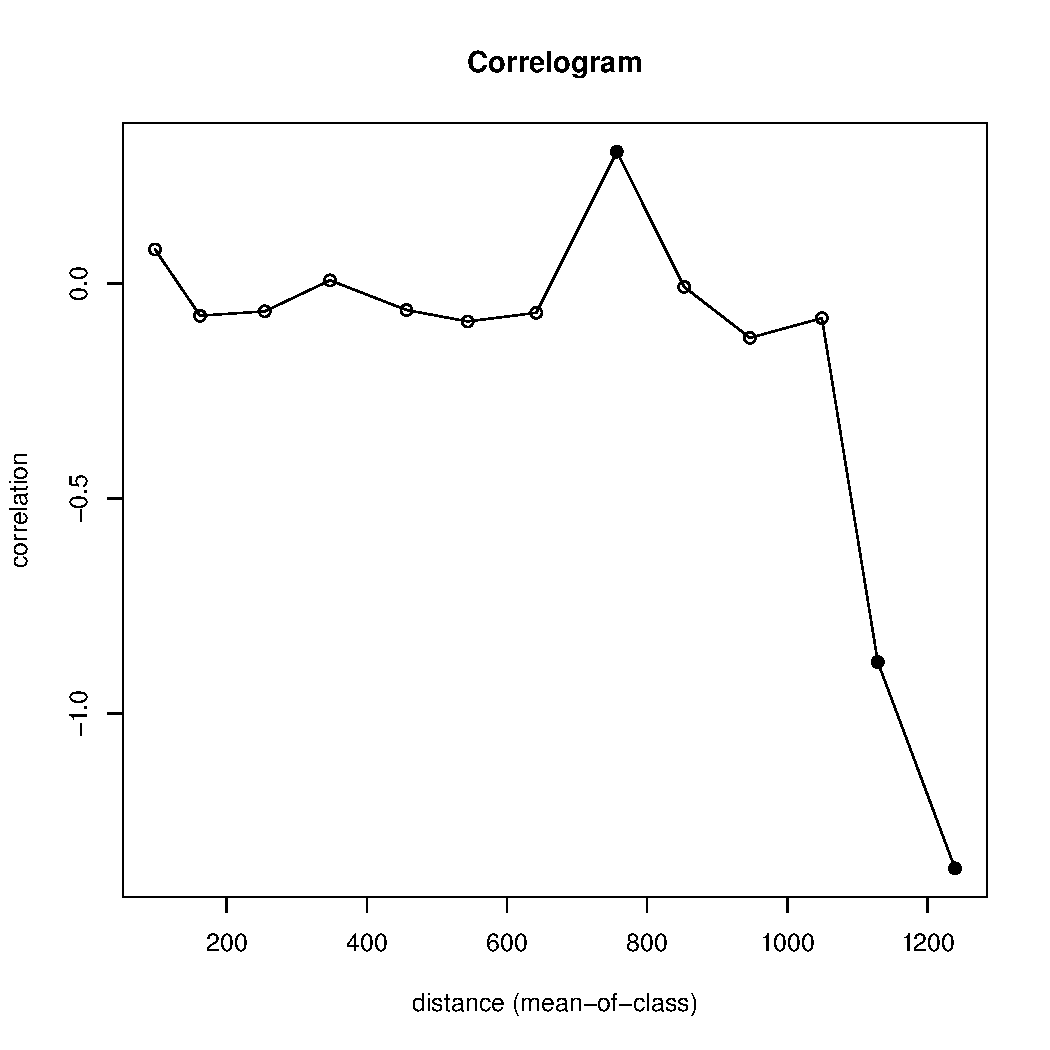
\includegraphics[width=65mm]{./Pala_macoma_age_N14_.pdf}
	\end{center}
	\end{minipage}

%	\caption{Микрораспределение макробентоса на литорали Дальнего пляжа г.~Дальнезеленецкая в 2007 году.}
%	\label{ris:moransI_Plyazh07_1}
	\end{figure}

\end{document}
